\section{Evaluation}
\label{sec:eval}

We evaluate the accuracy of the variants of our algorithm through a series of simulations in which we fine tune the various parameters: number of stages, memory size, and randomized admission policy coefficients. In order to simulate realistic streams of traffic, we ran testing using three different traces from the equinox chicago ISP backbone link, recorded in 2016. These anonymized traces each contain between 20 - 40 million packets, over 1 million different flows, and range from 40 minutes to 1 hour long. The data was obtained with permission from the Center for Applied Internet Data Analysis (CAIDA). We parsed the data from the CAIDA traces to isolate only the source IP addresses. Each source IP address is considered a separate flow.

\subsection{Accuracy Metrics}
In our experiments, we tested several combinations of the design techniques described above. We focused on testing the two different admission policies, and applied different levels of randomized ``hashing'' to find an optimal algorithm. When applying front rejection, we found that uniformly randomizing the table index in the first stage only yielded the best results, and gave a [INSERT percent] improvement over simple front rejection with normal hashing. While some randomization provided improvements for front rejection, our tests of back rejection showed that normal hashing at all stages was best. With these best versions identified, we moved on to comparing these algorithms with the standard HashPipe algorithm.

We began algorithm comparison by varying the available memory size, which corresponds to a greater number of counters that can be stored across all hash tables. Figure 2 shows our results when searching for the top 300 flows and using 6 table stages. Both algorithms that applied an admission policy outperformed the standard HashPipe algorithm for all tested memory sizes. Accuracy rates improved by about 20 percent when the number of counters was limited to 300, equal to the number of flows top-k flows being identified, and increases to more than 50 percent improvement when more than 2000 counters are used. In all algorithms, improvement begins to diminish after 1000 counters are available.


\begin{figure}[t]
  \centering
    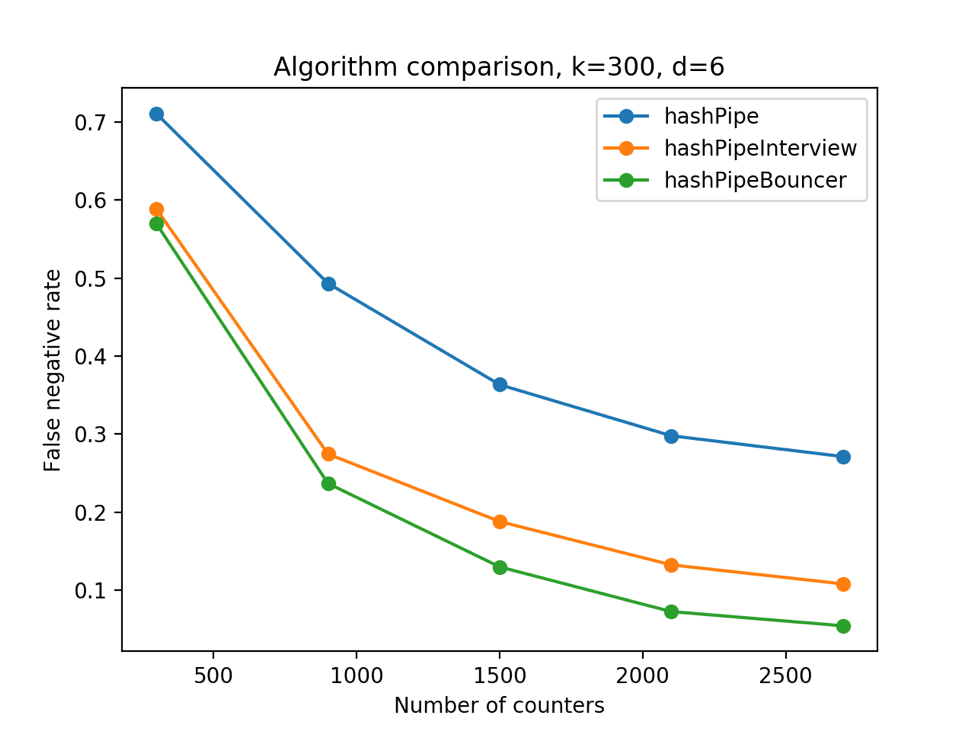
\includegraphics[scale=0.58]{algComparison}
     \caption{Comparison of false negatives of Interview and Bouncer to baseline. Both algorithm optimizations improve on the standard HashPipe algorithm over the entire tested memory range}
     \label{fig:bp-image}
\end{figure}

\begin{figure}[t]
  \centering
    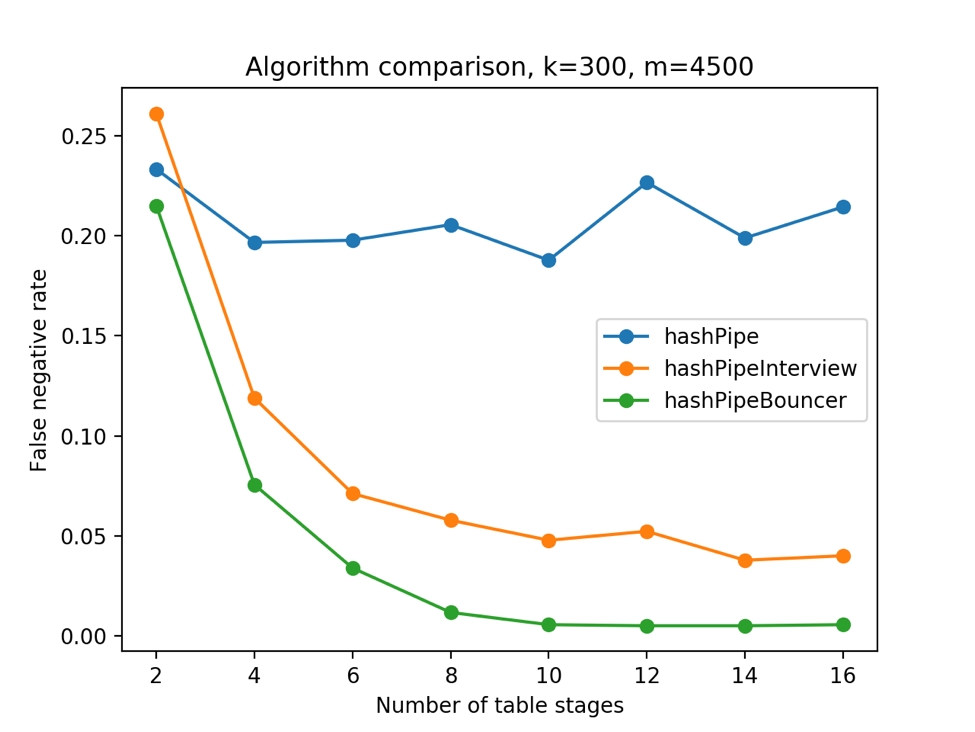
\includegraphics[scale=0.58]{stageComparison}
     \caption{Comparison of algorithms when number of table stages is varied. Interview and Bouncer do not suffer from the same accuracy drawbacks as the baseline when increasing the number of table stages}
     \label{fig:bp-image}
\end{figure}